\documentclass[8pt]{beamer}
\usepackage[utf8]{inputenc}
\usepackage{lmodern}
%\usepackage{subfig}
\usepackage{caption}

\setbeamertemplate{navigation symbols}{}

\usetheme{Warsaw}
\usecolortheme[RGB={32,69,96}]{structure}
\beamersetuncovermixins{\opaqueness<1>{75}}{\opaqueness<2->{55}}
\addtobeamertemplate{footline}{\hfill\insertframenumber/\inserttotalframenumber\hspace{2em}\null}
%\beamertemplatetransparentcovered


\newcommand {\framedgraphic}[2] {
    \begin{frame}{#1}
        \begin{center}
            \includegraphics[width=\textwidth,height=0.8\textheight,keepaspectratio]{#2}
        \end{center}
    \end{frame}
}

\title{Soutenance projet de programmation}
\subtitle{Génération Automatique de Texte}
\author{B. Barthés \\ A. Boumera \\ B. Guiomar \\ C. Pennarun \\ A. Wintringer}
\date{Mardi 16 Avril 2013}

\begin{document} 
\begin{frame}
\titlepage
\end{frame}

\section*{Introduction}
\begin{frame}\frametitle{Introduction}
\end{frame}


\section{Déroulement du logiciel}

\subsection{Administrateur}

\subsubsection{Base de données}
\begin{frame}{Base de données}
\begin{block}{Création de projet}
\begin{center}
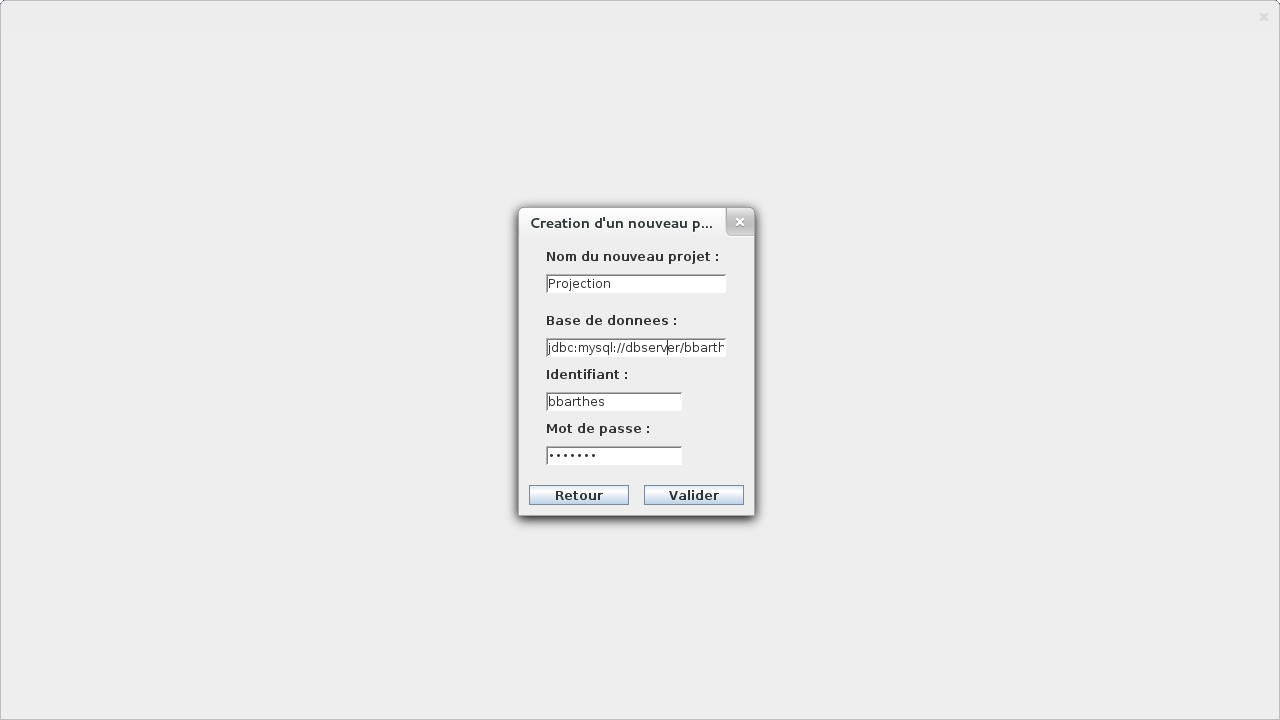
\includegraphics[scale=0.2]{db_connection.png}
\end{center}
\end{block}
\end{frame}

\begin{frame}{Base de données}
\begin{block}{Organisation de la base de données}
\begin{center}
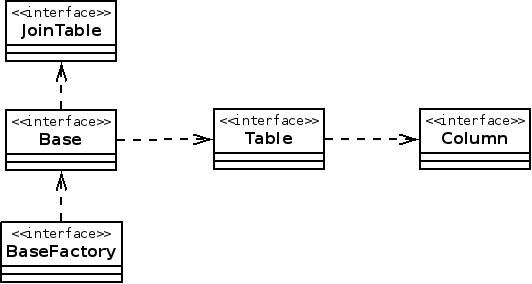
\includegraphics[scale=0.3]{db_presentation.png}
\end{center}
\end{block}
\end{frame}

\subsubsection{Base de données}
\begin{frame}{Base de données}
\begin{block}{Création de types}
\begin{center}
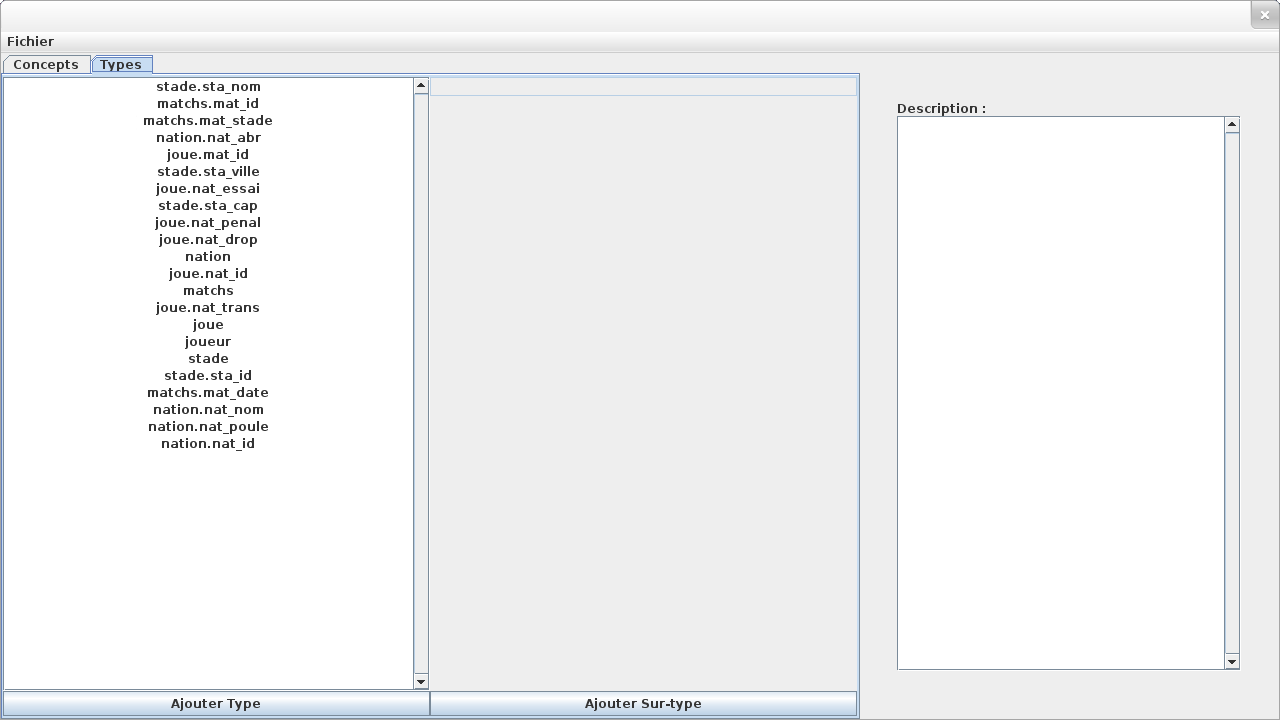
\includegraphics[scale=0.2]{creation_types.png}
\end{center}
\end{block}
\end{frame}


\subsubsection{Concepts et système de typage}
\begin{frame}{Concepts et système de typage}
\begin{columns}

\begin{column}{6cm}
\setbeamercovered{transparent}
\begin{itemize}[<+->]
\item Types
\\ \only<1>{Blabla types}
\item Concepts
\\ \only<2>{Blabla concepts}
\item Scénarios
\\ \only<3>{Blabla scénarios}
\end{itemize}
\end{column}

\begin{column}{6cm}
\only<1>{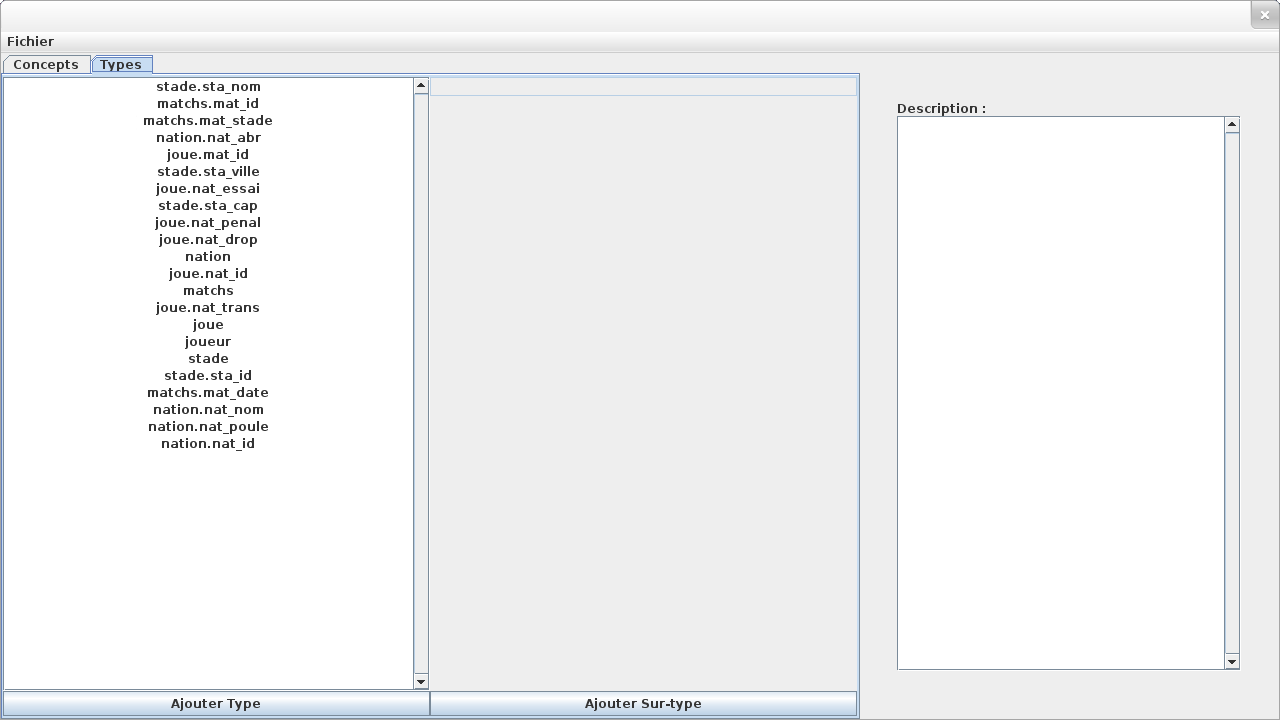
\includegraphics[scale=0.135]{creation_types.png}
\captionof{figure}[]{Fenêtre création de types}}

\only<2>{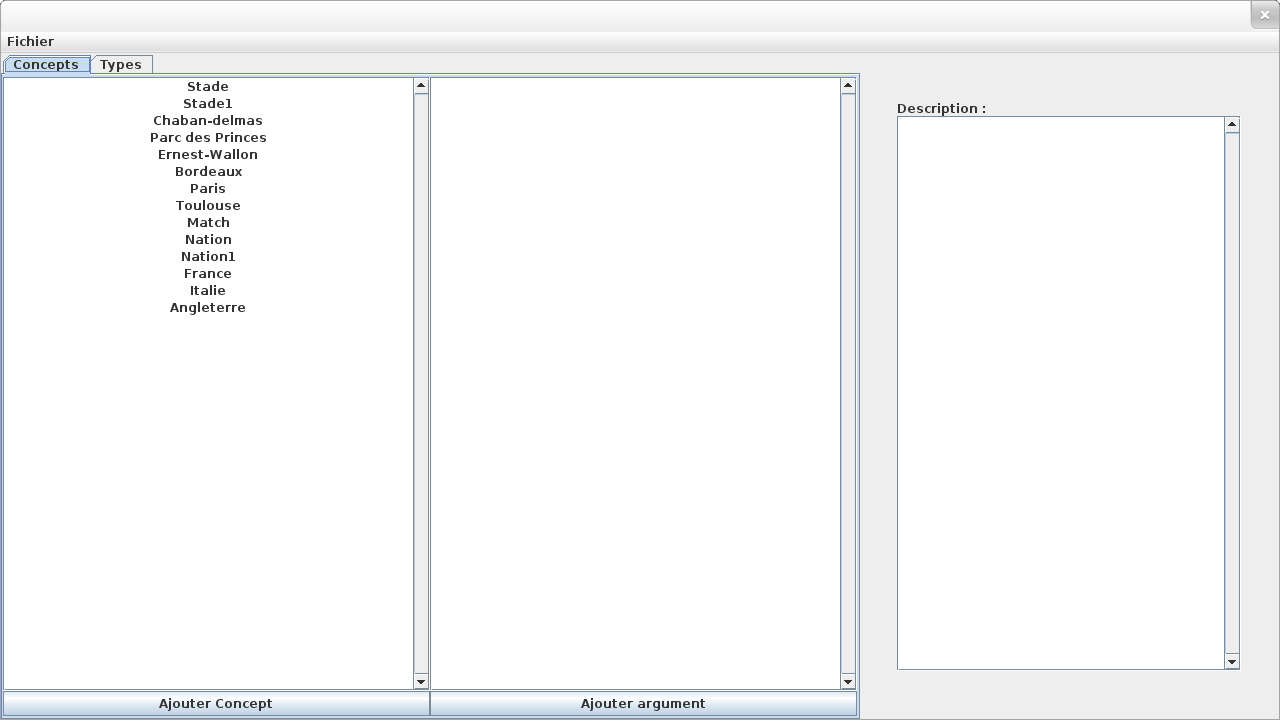
\includegraphics[scale=0.135]{creation_concepts.png}
\captionof{figure}[]{Fenêtre création de concepts}}

\only<3>{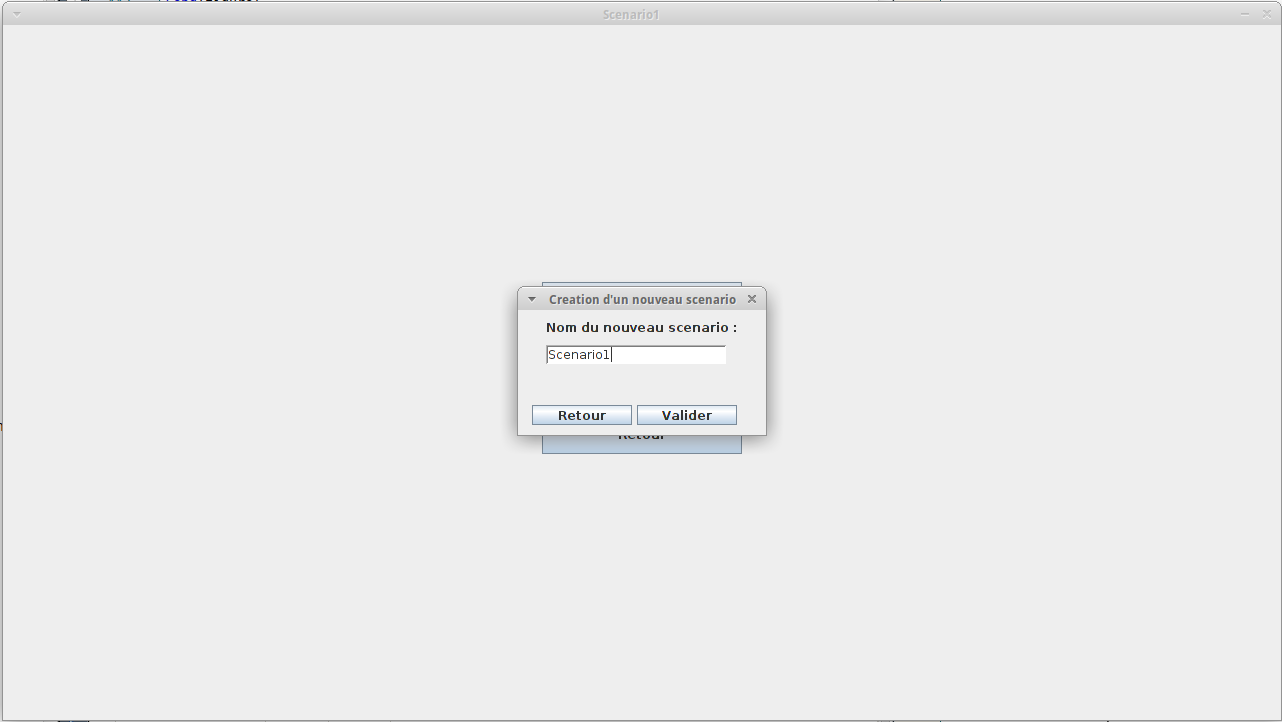
\includegraphics[scale=0.135]{creation_scenario.png}
\captionof{figure}[]{Fenêtre création de scénarios}}
\end{column}

\end{columns}
\end{frame}





\subsubsection{Sauvegarde}
\begin{frame}{Sauvegarde}
\end{frame}


\subsection{Utilisateur}

\subsubsection{Graphes conceptuels}
\begin{frame}{Graphes conceptuels}

\only<1-4>{
\uncover<1-4>{Point technique : rajout d'un noeud dans le graphe conceptuel}

\uncover<2-4>{\bigskip Problème : besoin d'une structure arborescente}
\uncover<3-4>{\\ MAIS plusieurs noeuds peuvent référencer le même Concept}

\uncover<4>{\bigskip Solution proposée : 
	\begin{itemize}
	\item utilisation d'un tag
	\item création d'une référence
	\end{itemize}
}
}

\only<5->{
\uncover<5->{addChild(GraphNode child, int index) sur un GraphNode parent}
\begin{itemize} 
\item \uncover<6->{on vérifie la compatibilité de child et parent}
\item \uncover<7->{si le noeud child est tagué}
				\uncover<8->{\\ on en crée une copie, qui en contient une référence}
				\uncover<9->{\\ on signale que child possède une référence}
\item  \uncover<10->{sinon, on met un tag dessus et on l'ajoute}
\end{itemize}

\uncover<11->{\bigskip Remarque : pas besoin de regarder les "enfants" du noeud à rajouter}
}
\end{frame}


\subsubsection{Connexion à Syntox}
\begin{frame}{Connexion à Syntox}
\begin{block}{Schéma de fonctionnement}
\begin{center}
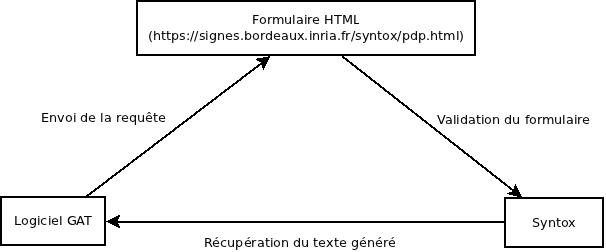
\includegraphics[scale=0.35]{syntox_connection.jpg}
\end{center}
Problème rencontré :
\begin{itemize}
\item Le résultat était incorrect.  \\
L'action du formulaire ne semblait pas s'activer.
\end{itemize}
\end{block}
\end{frame}



\section{Architecture}



\section{Test}
\begin{frame}
\end{frame}


\begin{frame}{Conclusion}
\section*{Conclusion}
\end{frame}


\end{document}
